\documentclass[a4paper,9pt]{article}

\usepackage[utf8]{inputenc}
\usepackage{graphicx}
\usepackage[francais]{babel}
%\usepackage{fullpage}
\usepackage{color}
\usepackage{array}

\begin{document}


\begin{titlepage}
\centering
\huge
\bfseries
Visualisation Scientifique\\[1\baselineskip]
\vspace{0.5cm}
\normalfont
\large
Interpolation et Visualisation de données avec Paraview\\[1\baselineskip]
	
\vspace{2cm}

\begin{figure}[!h]
\centering
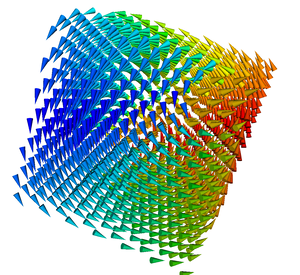
\includegraphics[width=0.9\textwidth]{couverture.png}
\end{figure}

\vspace{1.5cm}

\centering
\bfseries
\normalfont

\begin{tabular}{r c l}
Benjamin Aupetit & & Nicolas Cousin
\end{tabular}	

\vspace{0.5cm}

Ensimag\\
\textbf{\today}
\end{titlepage}

\clearpage
\newpage

\tableofcontents

\clearpage
\newpage

% INTRODUCTION

\section{Introduction}
\label{sec:introduction}

\section{Première Méthode : Shepard}
\label{sec:shepard}

\subsection{Description}
\label{subsec:shepard_description}

\subsection{Complexité}
\label{subsec:shepard_complexite}

\section{Deuxième Méthode : Multiquadriques de Hardy}
\label{sec:hardy}

\subsection{Description}
\label{subsec:hardy_description}

\subsection{Complexité}
\label{subsec:hardy_complexite}

\section{Implémentation}
\label{sec:implementation}

\subsection{Types utilisés}
\label{subsec:types}

\subsection{Implémentation de la méthode de Shepard}
\label{subsec:shepard_implementation}

\subsection{Implémentation de la méthode des multiquadriques de Hardy}
\label{subsec:hardy_implementation}

\section{Tests et Résultats}
\label{sec:tests_resultats}

\subsection{Visualisation de données avec Paraview}
\label{subsec:paraview}

\subsection{Présentation des méthodes de tests}
\label{subsec:presentation_tests}

\subsection{Validation de l'implémentation}
\label{subsec:validation_implementation}

\subsection{Tests Complexes}
\label{subsec:tests_complexes}

\subsection{Comparaison des deux méthodes]}
\label{subsec:comparaison_methodes}

\subsubsection{Temps de calcul}
\label{subsec:temps_calcul}

\subsubsection{Précision de l'interpolation}
\label{subsec:precision_interpolation}

\section{Conclusion}
\label{sec:conclusion}

\end{document}
